\documentclass[12pt,border=0pt]{standalone}

\usepackage[utf8]{inputenc} 
\usepackage{amssymb,amsmath}
\usepackage{tikz}
\usepackage{color}


\thispagestyle{empty}

\begin{document}

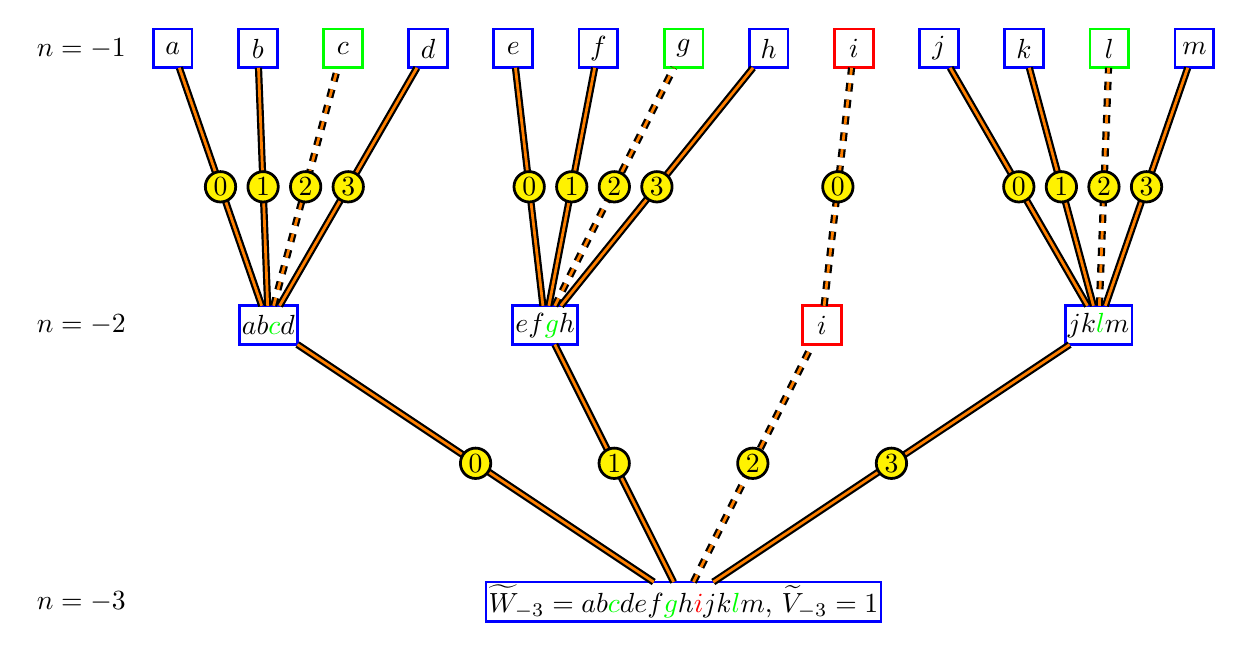
\begin{tikzpicture}[x=8pt,y=6pt]
  \centering
  \tikzset{VertexStyle/.style = {
    shape         = rectangle,
    draw          = blue, 
    fill          = white, 
  	line width    = 1pt, 
    text          = black,
    inner sep     = 1pt,
    outer sep     = 0pt,
    minimum size  = 14 pt,
    scale         = 1
    }
  }
  \tikzset{RedVertexStyle/.style = {
    shape         = rectangle,
    draw          = red, 
    fill          = white, 
  	line width    = 1pt, 
    text          = black,
    inner sep     = 1pt,
    outer sep     = 0pt,
    minimum size  = 14 pt,
    scale         = 1
    }
  }
  \tikzset{GreenVertexStyle/.style = {
    shape         = rectangle,
    draw          = green, 
    fill          = white, 
  	line width    = 1pt, 
    text          = black,
    inner sep     = 1pt,
    outer sep     = 0pt,
    minimum size  = 14 pt,
    scale         = 1
    }
  }
  \tikzset{EdgeStyle/.style = {
    draw            = black, 
    thick,
    double          = orange,
    double distance = 1pt
    }
  }
  \tikzset{EdgeStyleDashed/.style = {
    draw            = black,
    dashed, 
    thick,
    double          = orange,
    double distance = 1pt
    }
  }
  \tikzset{EdgeLabelStyle/.style = {
    draw          = black,
  	shape         = circle, 
  	line width    = 1pt, 
  	minimum size  = 10pt, 
    inner sep     = 1pt,
    outer sep     = 0pt,
    fill          = yellow,
    text          = black,
    scale         = 1
    }
  }

	\node[VertexStyle](A1) at (25, 0) {$\widetilde{W}_{-3}=ab{\color{green}c}def{\color{green}g}h{\color{red}i}jk{\color{green}l}m$, $\widetilde{V}_{-3}=1$};
	\node[VertexStyle](B1) at (6.25, 16.6666666666667) {$ab{\color{green}c}d$};
	\node[VertexStyle](B2) at (18.75, 16.6666666666667) {$ef{\color{green}g}h$};
	\node[RedVertexStyle](B3) at (31.25, 16.6666666666667) {$i$};
	\node[VertexStyle](B4) at (43.75, 16.6666666666667) {$jk{\color{green}l}m$};
	\node[VertexStyle](C01) at (1.92307692307692, 33.3333333333333) {$a$};
	\node[VertexStyle](C02) at (5.76923076923077, 33.3333333333333) {$b$};
	\node[GreenVertexStyle](C03) at (9.61538461538462, 33.3333333333333) {$c$};
	\node[VertexStyle](C04) at (13.4615384615385, 33.3333333333333) {$d$};
	\node[VertexStyle](C05) at (17.3076923076923, 33.3333333333333) {$e$};
	\node[VertexStyle](C06) at (21.1538461538462, 33.3333333333333) {$f$};
	\node[GreenVertexStyle](C07) at (25, 33.3333333333333) {$g$};
	\node[VertexStyle](C08) at (28.8461538461539, 33.3333333333333) {$h$};
	\node[RedVertexStyle](C09) at (32.6923076923077, 33.3333333333333) {$i$};
	\node[VertexStyle](C10) at (36.5384615384615, 33.3333333333333) {$j$};
	\node[VertexStyle](C11) at (40.3846153846154, 33.3333333333333) {$k$};
	\node[GreenVertexStyle](C12) at (44.2307692307692, 33.3333333333333) {$l$};
	\node[VertexStyle](C13) at (48.0769230769231, 33.3333333333333) {$m$};
	\draw[EdgeStyle](A1) to node[EdgeLabelStyle]{$0$} (B1);
	\draw[EdgeStyle](A1) to node[EdgeLabelStyle]{$1$} (B2);
	\draw[EdgeStyleDashed](A1) to node[EdgeLabelStyle, solid]{$2$} (B3);
	\draw[EdgeStyle](A1) to node[EdgeLabelStyle]{$3$} (B4);
	\draw[EdgeStyle](B1) to node[EdgeLabelStyle]{$0$} (C01);
	\draw[EdgeStyle](B1) to node[EdgeLabelStyle]{$1$} (C02);
	\draw[EdgeStyleDashed](B1) to node[EdgeLabelStyle, solid]{$2$} (C03);
	\draw[EdgeStyle](B1) to node[EdgeLabelStyle]{$3$} (C04);
	\draw[EdgeStyle](B2) to node[EdgeLabelStyle]{$0$} (C05);
	\draw[EdgeStyle](B2) to node[EdgeLabelStyle]{$1$} (C06);
	\draw[EdgeStyleDashed](B2) to node[EdgeLabelStyle, solid]{$2$} (C07);
	\draw[EdgeStyle](B2) to node[EdgeLabelStyle]{$3$} (C08);
	\draw[EdgeStyleDashed](B3) to node[EdgeLabelStyle, solid]{$0$} (C09);
	\draw[EdgeStyle](B4) to node[EdgeLabelStyle]{$0$} (C10);
	\draw[EdgeStyle](B4) to node[EdgeLabelStyle]{$1$} (C11);
	\draw[EdgeStyleDashed](B4) to node[EdgeLabelStyle, solid]{$2$} (C12);
	\draw[EdgeStyle](B4) to node[EdgeLabelStyle]{$3$} (C13);

  \node at (-2.20, 33.3333333333333)  {$n=-1$};
  \node at (-2.20, 16.6666666666667) {$n=-2$};
  \node at (-2.20, 0) {$n=-3$};


  \end{tikzpicture}

\end{document}
